\documentclass[WHATMANUAL.tex]{subfiles}

\begin{document}

\chapter{Creating a Weather Station List Manually}
\label{app:custom_station_list}

WARNING: this section needs to be updated and revised.

The stations information need to be saved in a tabular-separated values text file with an “lst” extension. A template of a station list (station\_list\_template.lst) is provided with the program in the Zip archive and an example is presented in Error: Reference source not found. The fields Station Name, Year, Start, Year End and Province do not need to match strictly with the station's URL. These fields can be assigned any name/value by the user and are not directly used in the downloading process of weather data. The only field that is directly used in the download process is Station ID that is a unique number attributed to each weather station.

Once a file containing a list of weather stations' information has been created, it is possible to load it in Rainbird by clicking on the  Load button located in the Fetch and Merge tab (Error: Reference source not found). The station list can be refreshed at any time by clicking on the  Refresh button.

\begin{figure}[h!]
\centering
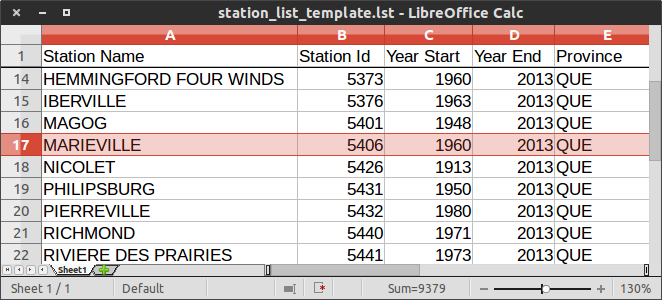
\includegraphics[width=0.5\textwidth]{img/example_staList}
\caption[Weather Station List (*.lst) Sample]{Weather Station List (*.lst) Sample}
\label{fig:example_staList}
\end{figure}

\paragraph{Step 1} First go to \url{www.climate.weather.gc.ca}.

\paragraph{Step 2} At the bottom of the page, click on Advanced Search (see the red arrow in Figure~\ref{subfig:customWeaterStaList_step1}).

\paragraph{Step 3} Search for a station either by Province, Name or Proximity. For this example, the search was made using the Name of the station (see Figure A2).

\paragraph{Step 4} The research yielded one result (Figure A3). For Data Interval, select Daily and click Go.
	WARNING: The downloading and formatting of Hourly data is not currently supported in WHAT (but could be in a future version of the software).

\paragraph{Step 5} The URL associated with Marieville weather station is:\vspace{0.5cm}

\begin{sloppypar}
\noindent
\url{http://climate.weather.gc.ca/climateData/dailydata_e.html?timeframe=2&Prov=QUE&StationID=5406&dlyRange=1960-06-01|2013-12-31&Year=2013&Month=12&Day=01}.
\end{sloppypar}\vspace{0.5cm}

From this URL, we find that its Station ID is 5406 (see red circle in Figure A4), that is located in the province of Quebec (QUE) and that data are available from 1960 to 2013.

\begin{figure}[h!]
        \centering
        \begin{subfigure}[t]{0.45\textwidth}
                \centering
                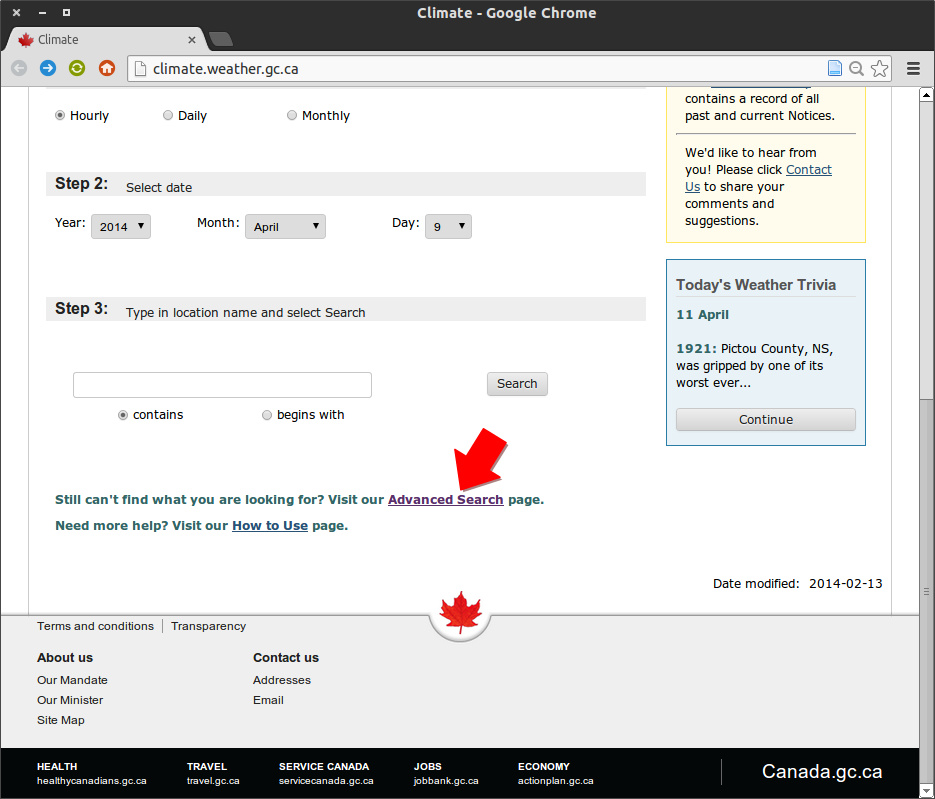
\includegraphics[width=\textwidth]{img/customWeaterStaList_step1}
                \caption{Step 1}
                \label{subfig:customWeaterStaList_step1}                
        \end{subfigure}%
        \hspace{0.5cm}
        \begin{subfigure}[t]{0.45\textwidth}
                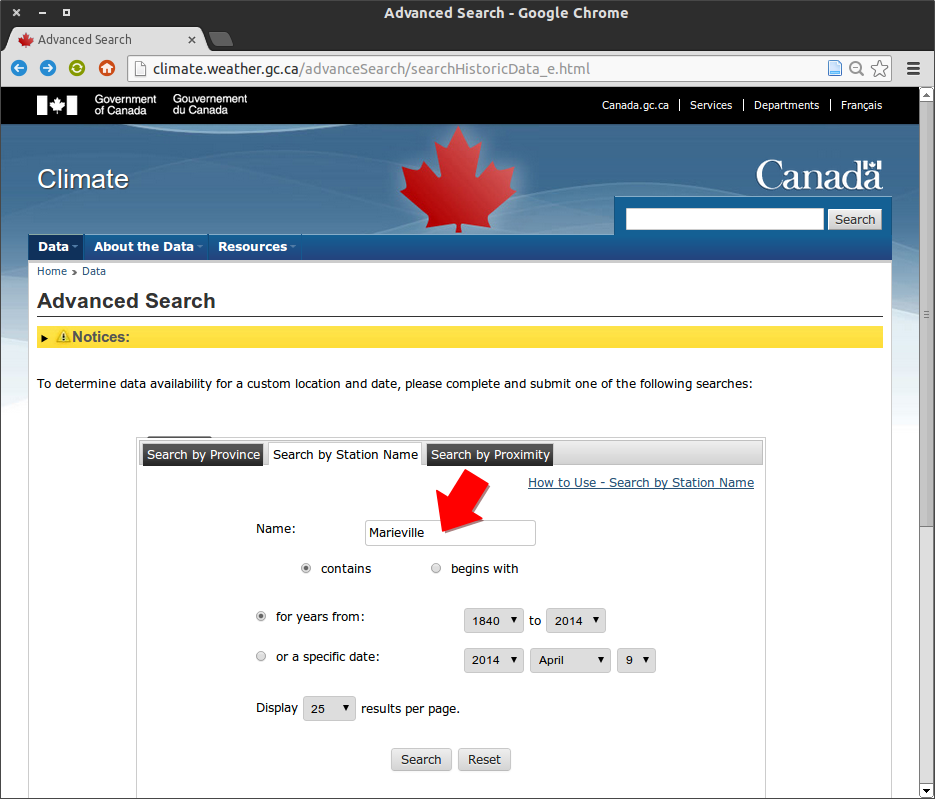
\includegraphics[width=\textwidth]{img/customWeaterStaList_step2}
                \caption{Step 2}
                \label{subfig:customWeaterStaList_step2}
        \end{subfigure}
        \\[0.5cm]
        \begin{subfigure}[t]{0.45\textwidth}
                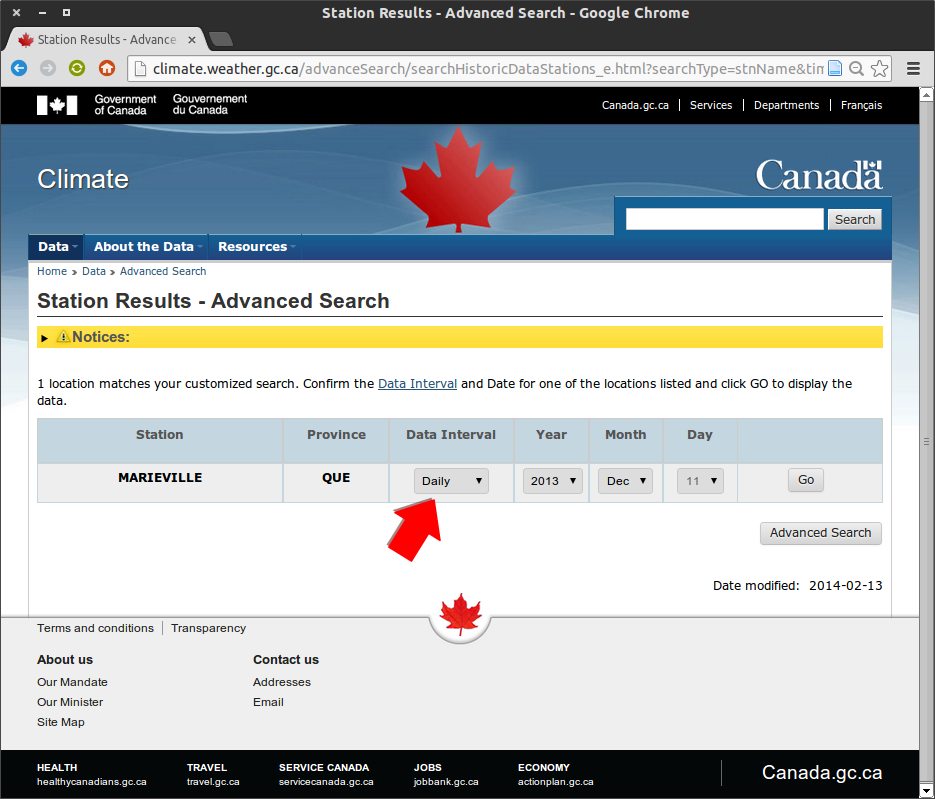
\includegraphics[width=\textwidth]{img/customWeaterStaList_step3}
                \caption{Step 3}
                \label{subfig:customWeaterStaList_step3}
        \end{subfigure}
        \hspace{0.5cm}
        \begin{subfigure}[t]{0.45\textwidth}
                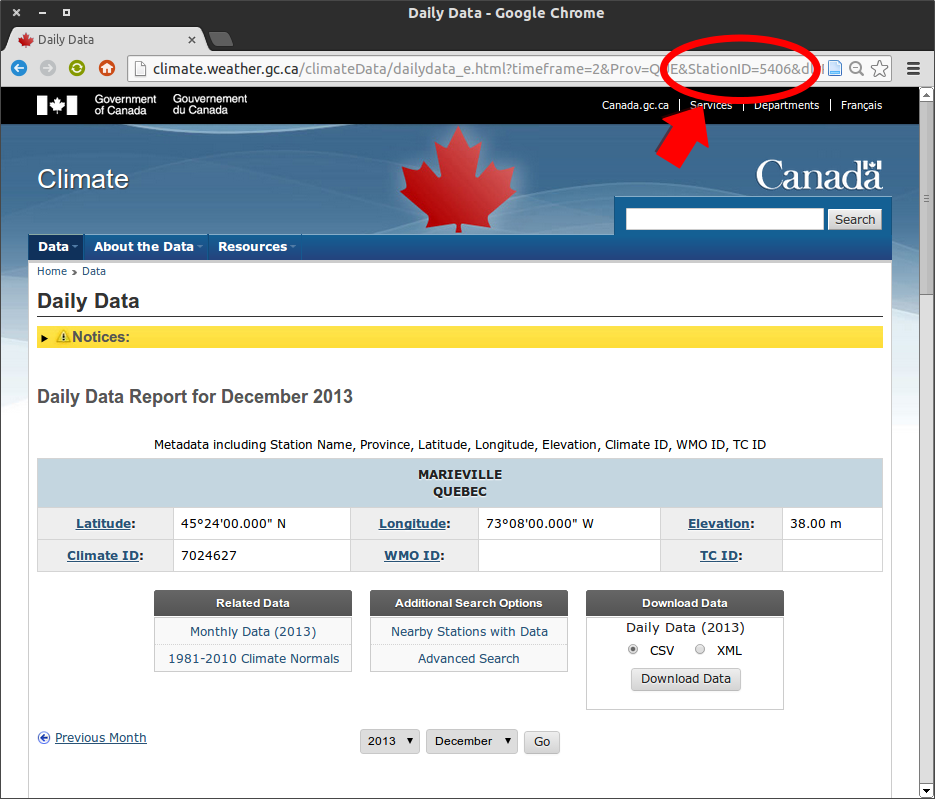
\includegraphics[width=\textwidth]{img/customWeaterStaList_step4}
                \caption{Step 4}
                \label{subfig:customWeaterStaList_step4}
        \end{subfigure}
        \caption[Creation of a custom weather station list how-to]{Creation of a custom weather station list how-to}\label{fig:customStaList_Howto}
\end{figure}

\end{document}